\documentclass{beamer}

\title{Section 1}
\author{TA: Dante Buhl}
\institute{UCSC Math-19B}
%\date{Week 2}
\graphicspath{ {./images/} }
%\usepackage{xcolor}
\usepackage{verbatim}
\usetheme{Berkeley}
\usecolortheme{spruce}
\usefonttheme{serif}
%\usepackage[x11names]{xcolor}
\usepackage{amsmath}
\usepackage{pifont}


\begin{document}

\newcommand{\bmp}[1]{\begin{minipage}{#1\textwidth}}
\newcommand{\emp}{\end{minipage}}


%Title
\frame{\titlepage}

\section{Welcome to Section!}
\begin{frame}{Plan for Today}
    Topics to Cover
    \begin{itemize}
        \item Introductions and forming groups
        \item Review Activity
    \end{itemize}
    Section Activity 1
    \begin{itemize}
        \item 3 questions
    \end{itemize}
    Assignments
    \begin{itemize}
        \item Homework 1 (Due Fri, Jan. $19^{th}$)
    \end{itemize}
\end{frame}

\begin{frame}{Introductions}
    Hello! I'm Dante. 
    \vspace{10pt}

    \bmp{.4}
        About Me:
        \begin{itemize}
            \item graduate student in Applied Math
            \item 22 years old
            \item Play guitar
            \item Have two pet snakes
            \item Researcher in Fluid Dynamics
        \end{itemize}
    \emp
    \hspace{5pt}
    \bmp{.55}
        \centering
        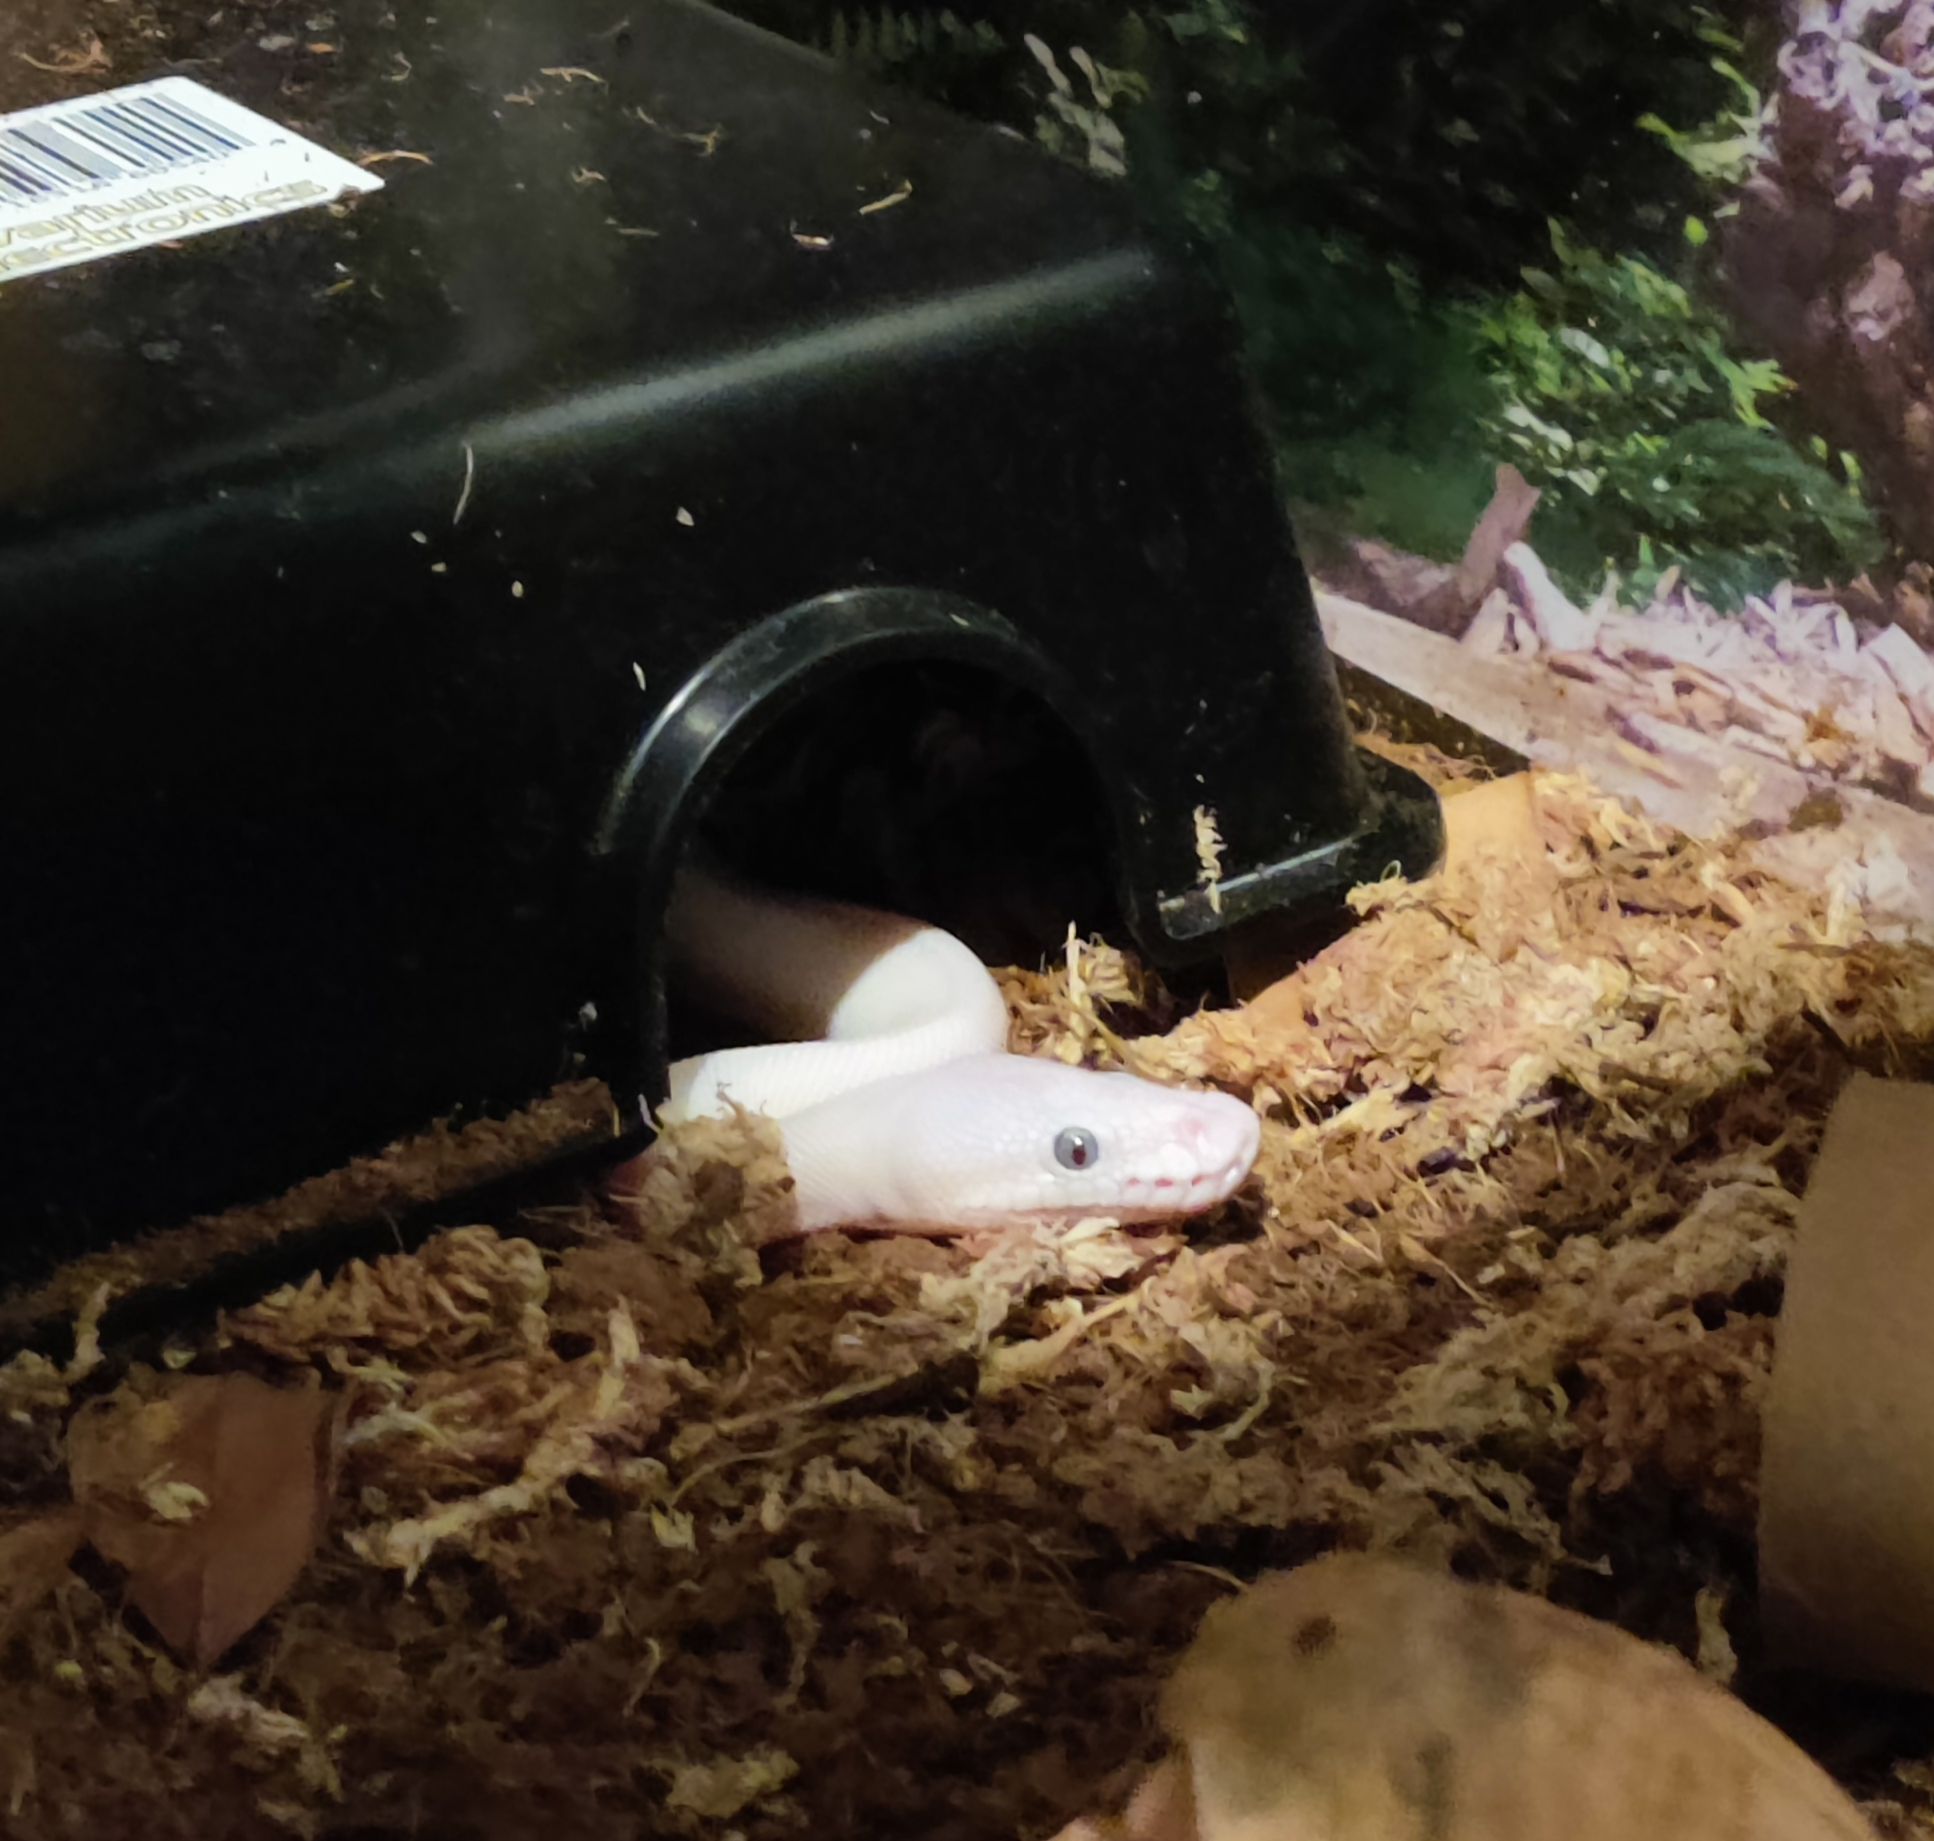
\includegraphics[width=.75\textwidth]{duncan.jpg}
    \emp
\end{frame}

\begin{frame}{Get to know your classmates}
    \bmp{.4}
    Go meet 5 new people and ask them about their winter break and how they feel today on the animal scale :). 

    \emp
    \hspace{3pt}
    \bmp{.55}
    \begin{center}
        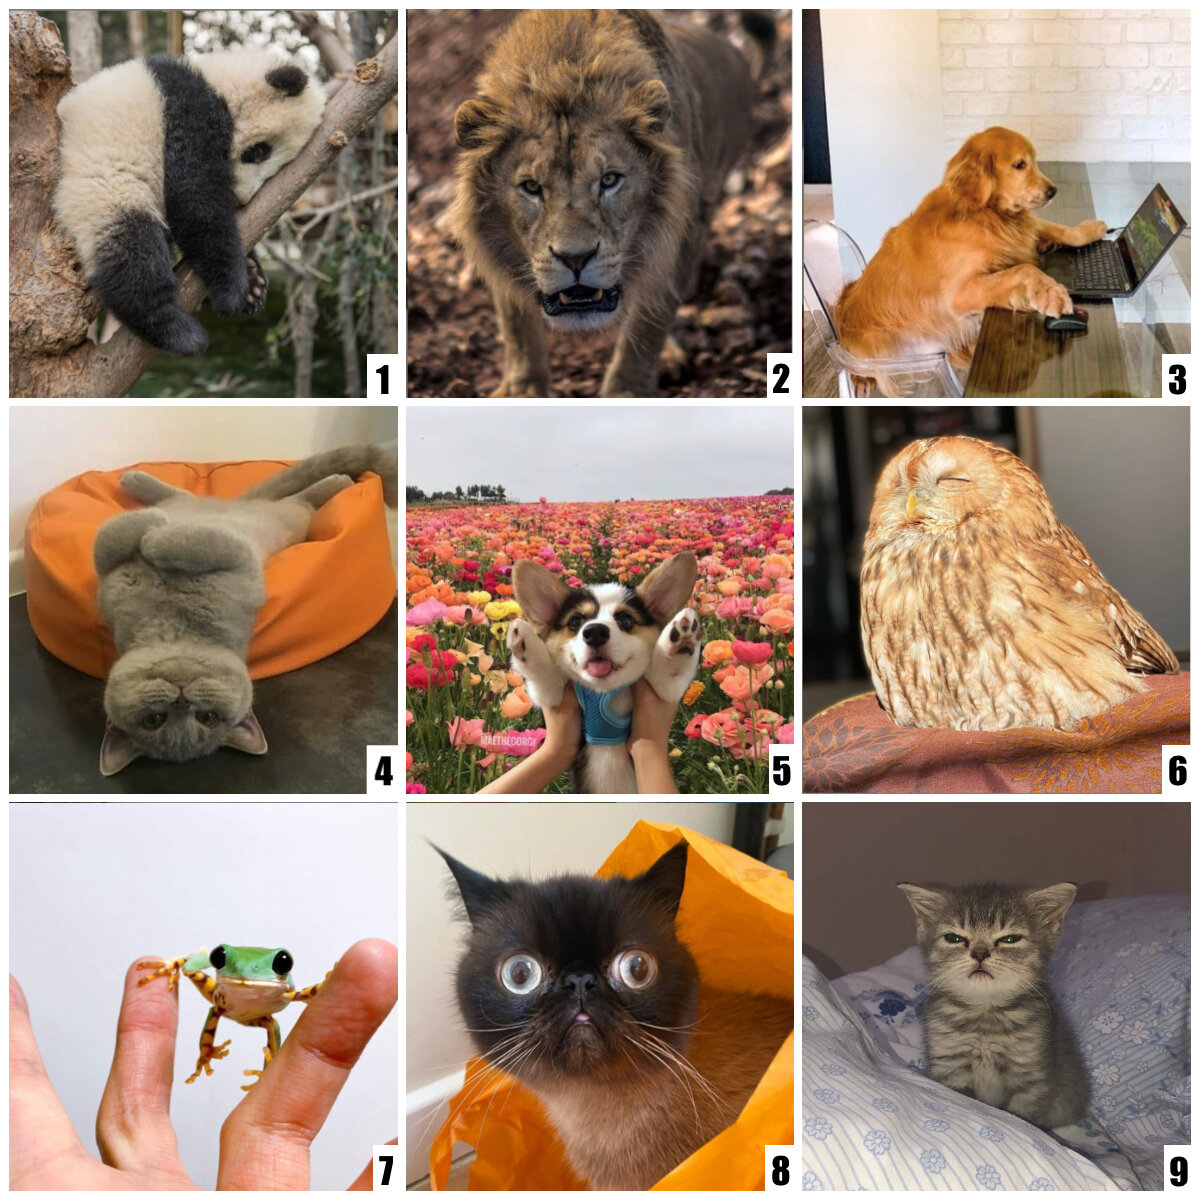
\includegraphics[width=\textwidth]{animalscale.jpeg}
    \end{center}
    \emp

    NOTE: Think about people you might want to form "working groups" with. 
\end{frame}

\begin{frame}{Learning Outcomes}
    \begin{itemize}
        \item Understanding how to recognize and compute the value of signed area under curves.
        \item Differentiating different area under curve approximations and how to construct them. 
        \item Applying Linearity to the sums, limits, and integrals.
    \end{itemize}
\end{frame}

\section{Practice}
\begin{frame}{Review Activity}

    
\includegraphics[width=.6\textwidth]{activity.png}

Or you can find it in canvas files in section materials titled reviewactivity1.pdf    

\end{frame}


\begin{frame}{Section Activity 1 (Access Code: 117f1)}

\[
    p = \rho g h
\]
\[
    l = 154 m, h = 11 m, \rho = 970.56 Kg/m^3
\]
\[ g = 9.8 m/s^2 \]
\[ F = p A\]
    
\end{frame}

\end{document}
